\subsection{Convolutional Neural Network (CNN)}
\textit{Deep Learning} berarti jaringan saraf (\textit{neural network} yang memiliki banyak lapisan tersembunyi (\textit{hidden layers}. Kedalaman atau jumlah lapisan ini memungkinkan sebuah jaringan mempelajari representasi fitur yang semakin abstrak Secara matematis, jika sebuah neuron menerima vektor masukan 
$$
\mathbf{x} = (x_1, x_2, \ldots, x_n)^\top
$$
dengan bobot
$$
\mathbf{w} = (w_1, w_2, \ldots, w_n)^\top
$$
dan bias $b$, maka keluarannya $z$ dapat ditulis sebagai
$$
z = \sigma(\mathbf{w}^\top \mathbf{x} + b),
$$

Proses pembelajaran dilakukan dengan meminimalkan fungsi \textit{loss} menggunakan algoritma optimasi dengan cara menyesuaikan bobot dan bias agar keluaran jaringan mendekati target yang diinginkan. 

Convolutional Neural Network (CNN) adalah jenis \textit{deep neural network} yang dirancang khusus untuk memproses data yang memiliki struktur spasial, seperti citra dua dimensi. Berbeda dengan jaringan saraf berlapis penuh (fully-connected network) yang menghubungkan setiap neuron pada satu lapisan ke semua neuron di lapisan berikutnya, CNN menggunakan operasi konvolusi dengan filter (kernel) berukuran kecil yang digeser (sliding) di atas citra atau \textit{feature maps}.

Pada sebuah \textit{convolutional layer}, diberikan tensor masukan berdimensi
$$
H \times W \times C_\text{in},
$$
serta sekumpulan filter berukuran kecil (misalnya $3 \times 3$) dengan $C_\text{out}$ buah filter. Setiap filter menghasilkan satu \textit{feature map}, sehingga keluaran layer ini berupa tensor
$$
H' \times W' \times C_\text{out},
$$
di mana $H'$ dan $W'$ adalah tinggi dan lebar baru setelah operasi konvolusi (dan mungkin subsampling). Intuisi utama CNN adalah bahwa setiap filter belajar mendeteksi pola tertentu (misalnya tepi, tekstur, atau bentuk) pada berbagai lokasi spasial.

\begin{figure}[H]
    \centering
    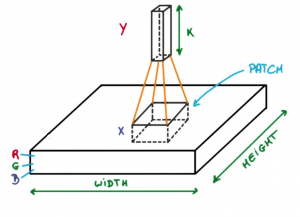
\includegraphics[width=0.4\textwidth]{assets/contoh-cnn.png}
    \caption{\href{https://www.geeksforgeeks.org/machine-learning/introduction-convolution-neural-network/}{Visualisasi \textit{Convolutional Layer}}}
    \label{fig:contoh-cnn}
\end{figure}


Sebuah Convolutional Neural Network (CNN) tersusun atas urutan beberapa lapisan, di mana setiap lapisan mengubah sebuah volume data tensor menjadi volume lain melalui fungsi yang terdiferensialkan. Untuk citra, volume ini biasanya memiliki dimensi tinggi, lebar, dan kanal (\textit{channel}) atau $H \times W \times C$.

\begin{IEEEitemize}
    \item \textit{Input layer}. Layer ini menampung data mentah yang diberikan ke jaringan. Pada lapisan ini belum ada komputasi selain penyediaan data untuk lapisan berikutnya.
    \item \textit{Convolutional layer}. Layer ini bertugas mengekstraksi fitur dari citra. Lapisan ini memiliki sekumpulan filter (kernel) berukuran kecil, misalnya $3 \times 3$ yang digeser di atas citra. Untuk setiap posisi, filter dan \textit{patch} citra yang bersesuaian dikalikan elemen per elemen, lalu dijumlahkan, menghasilkan satu nilai pada pada \textit{feature map}
    \item \textit{Activation layer}. Layer ini menerapkan fungsi aktivasi nonlinier pada tiap elemen pada keluaran \textit{convolutional layer}. Fungsi aktivasi yang umum digunakan, yaitu ReLU.
        $$
        \text{ReLU}(x) = \max(0, x)
        $$
    Lapisan ini tidak mengubah dimensi volume, tetapi penting agar jaringan memodelkan hubungan nonlinier yanag kompleks antar piksel.

    \item \textit{Pooling Layer}. Layer ini disisipkan secara berkala untuk mengecilkan ukuran dari \textit{feature maps}. Konsep utamanya adalah untuk merangkum informasi lokal di suatu submatrix kecil menjadi satu nilai. Dua jenis \textit{pooling} yang paling sering digunakan adalah \textit{max pooling} yang mengambil nilai maksimum dalam submatrix dan \textit{average pooling} yang mengambil nilai rata-rata dalam submatrix. 

    \item \textit{Flattening} dan \textit{fully connected layer}. Setelah beberapa kali konvolusi-aktivasi-pooling, biasanya volume fitur yang tersisa diubah menjadi vektor satu dimensi agar dapat dihubungkan ke lapisan \textit{fully connected}. Jika volume terakhir memiliki ukuran $H_f \times W_f \times C_f$, maka hasil flatten adalah vektor di $\mathbb{R}^{H_f \cdot W_f \cdot C_f}$. Lapisan ini kemudian memperlakukan vektor ini seperti masukan jaringan saraf biasa. Setiap neuron terhubung ke semua komponen vektor, dengan bobot dan bias masing-masing. Lapisan ini digunakan untuk klasifikasi, regresi, atau tujuan akhir lainnya. 

    \item \textit{Output layer}. Layer terakhir ini menerima keluaran dan mengubahnya menjadi bentuk yang sesuai dengan tugas.

\end{IEEEitemize}

\begin{figure}[H]
    \centering
    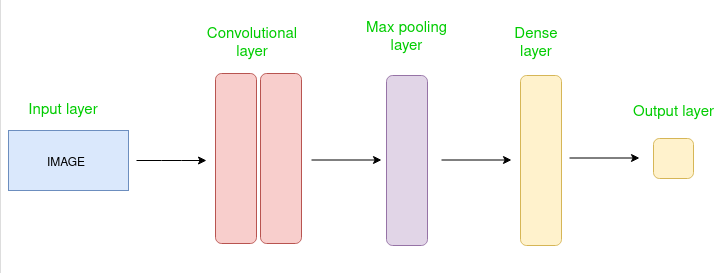
\includegraphics[width=0.4\textwidth]{assets/cnn-architecture.png}
    \caption{\href{https://www.geeksforgeeks.org/machine-learning/introduction-convolution-neural-network/}{Arsitektur CNN}}
    \label{fig:arsitektur-cnn}
\end{figure}

Dalam algoritma NST, arsitektur CNN yang digunakan adalah VGG-19. Baca: \url{https://www.sciencedirect.com/topics/computer-science/vgg-19-convolutional-neural-network} sebagai referensi
